\chapter{Observaties}
In dit hoofdstuk worden de resultaten getoond van de testen die zijn uitgevoerd. Deze resultaten zullen in dit hoofdstuk enkel getoond worden met een bespreking van de speciale elementen. Er zullen nog geen conclusies gemaakt worden, dit wordt in het volgende hoofdstuk gedaan. 

De resultaten zullen besproken worden per testsoort: eerst de resultaten voor de calibratie daarna voor beschikbaarheid en tenslotte voor consistentie. 

De ruwe testdata kan geraadpleegd worden op \url{https://github.com/thuys/YCSB-Testdata}. 

\section{Calibratie}

\paragraph{Aantal gebruikers}
De resultaten van de calibratietest voor het aantal gebruikers kunnen gevonden worden in figuur \ref{fig:calibratie-gebruikers-resultaat}. Op de x-as is het gemiddeld aantal queries per second getoond over een periode van 600s, op de y-as de gemiddelde vertraging. De verschillende punten stellen een aantal gebruikers voor die zijn aangegeven met het bijhorend getal. 

Het aantal gebruikers wordt zo gekozen dat het totale aantal queries zakt of voor een sterke groei in vertraging zorgt, dit zorgt voor de gegevens in tabel \ref{table:calibratie-gebruikers-resultaat}. \todo{Check data in tabel}

\begin{table}[h!]
	\centering
	\begin{tabular}{l| l }
		\textbf{DBMS} & Aantal gebruikers \\
		\hline
		HBase & 40 \\
		MongoDB & 15\\
		Pgpool-II & 30\\
	\end{tabular}
	\caption{Calibratie: Aantal gebruikers per test voor de verschillende DBMS's}
	\label{table:calibratie-gebruikers-resultaat}
\end{table}

\begin{figure}[h!] 
\centering
	\subfigure[MongoDB]{\label{fig:calibratie-gebruikers-mongodb} \includegraphics[width=0.8\textwidth]{img/Observaties/threads-MongoDB}}
	\subfigure[Pgpool-II]{\label{fig:calibratie-gebruikers-pgpool-ii} 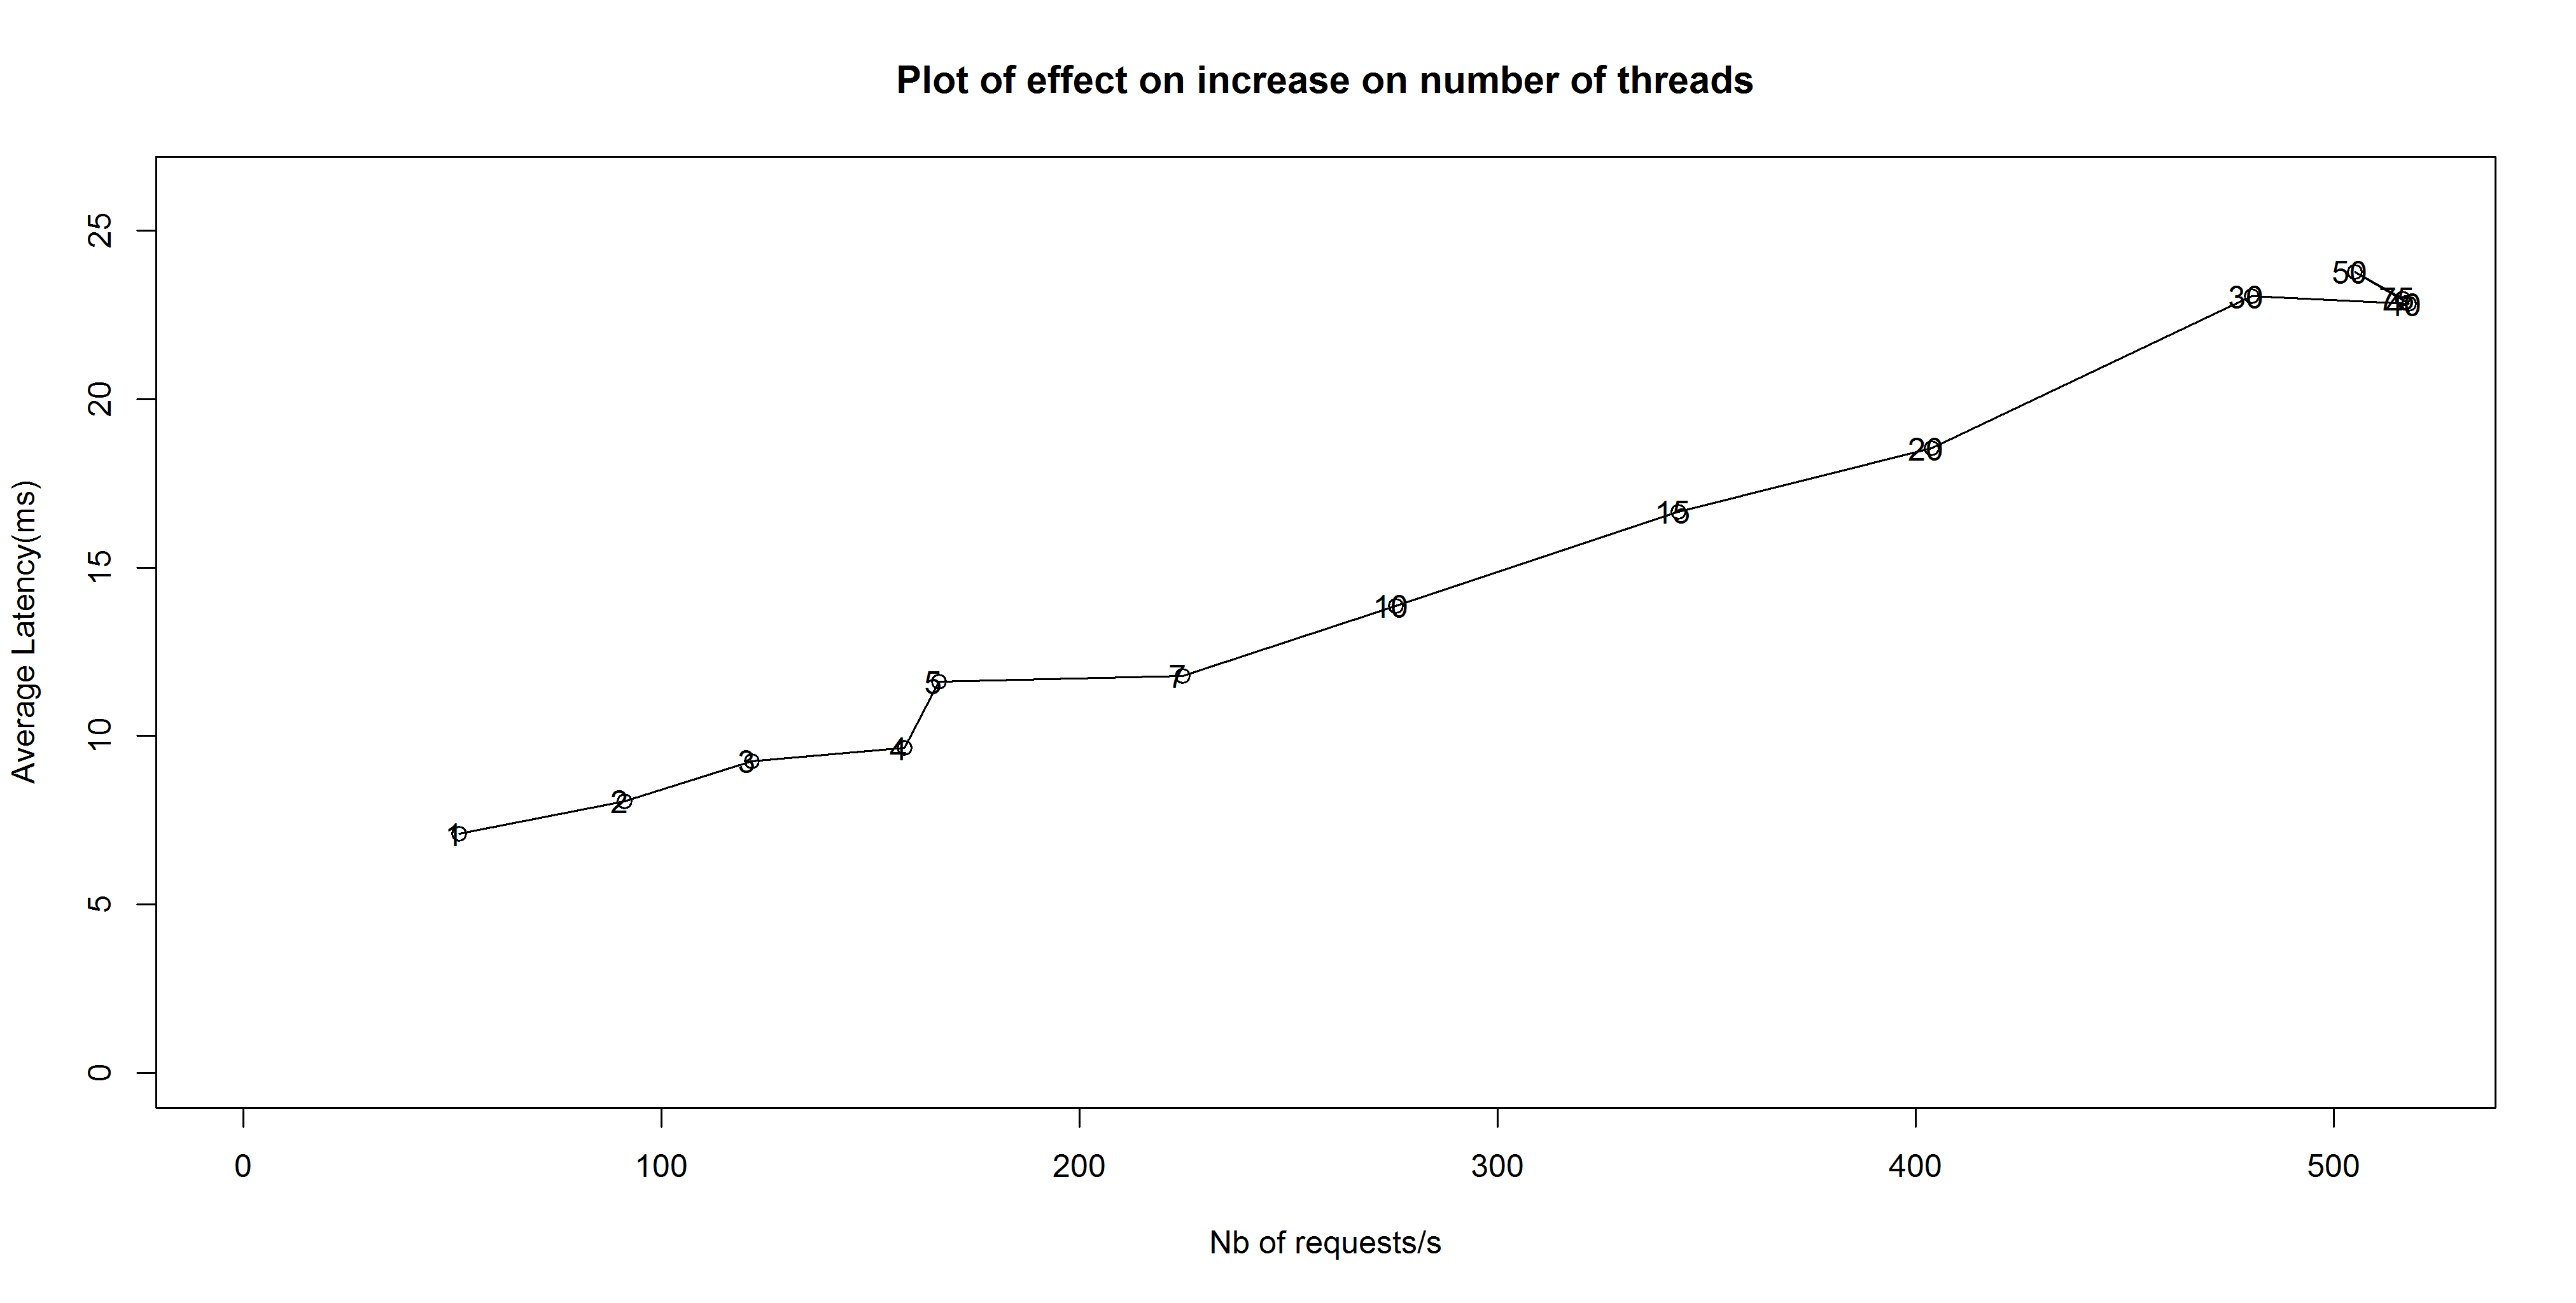
\includegraphics[width=0.80\textwidth]{img/Observaties/threads-postgresql}}
	\subfigure[HBase]{\label{fig:calibratie-gebruikers-hbase} \includegraphics[width=0.8\textwidth]{img/Observaties/threads-HBase}}
	\caption{Calibratie: Overzicht van het aantal requests tot de gemiddelde vertraging voor verschillend aantal gebruikers. Elk datapunt stelt een verschillend aantal gebruikers voor met het aantal rechtsboven het punt. }
	\label{fig:calibratie-gebruikers-resultaat}
\end{figure}

\paragraph{Aantal queries per seconde}
De resultaten voor de calibratietest voor het aantal queries per seconden kunnen gevonden worden in de figuren \ref{fig:calibratie-queriesperseconde-hbase}, \ref{fig:calibratie-queriesperseconde-mongodb} en \ref{fig:calibratie-queriesperseconde-pgpool-ii} voor respectievelijk HBase, MongoDB en Pgpool-II. Deze figuren tonen in de bovenste figuur de gemiddelde vertraging op een query afhankelijk van het aantal queries per seconde, zoals te verwachten stijgt de trendlijn hierdoor. De onderste figuur toont op de y-as de verhouding tussen het eigenlijk aantal uitgevoerde queries per seconde t.o.v. het gevraagde aantal queries per seconde. Bij het vragen van 100 queries/sec wordt er in de praktijk bijvoorbeeld maar 60 uitgevoerd, dit zorgt voor een waarde $0.6$. 

Met beide figuren samen, kan een matige belasting gekozen. Een matige belasting is een belasting waarbij de onderste figuur de waarde 1 zo dicht mogelijk benaderd en de vertraging nog niet te veel is gestegen t.o.v. van een lage belasting. De gekozen waarde zijn te vinden in tabel \ref{table:calibratie-queriesperseconde-resultaat}.  \todo{Check data in tabel}

\begin{table}[h!]
	\centering
	\begin{tabular}{l| l }
		\textbf{DBMS} & Aantal requests per seconde \\
		\hline
		HBase & 200 \\
		MongoDB & 200\\
		Pgpool-II & 100\\
	\end{tabular}
	\caption{Calibratie: Aantal queries per seconde per test bij een matige belasting voor de verschillende DBMS's.}
	\label{table:calibratie-queriesperseconde-resultaat}
\end{table}

\begin{figure}[h!] 
	\centering
	\subfigure{\label{fig:calibratie-queriesperseconde-hbase-1} 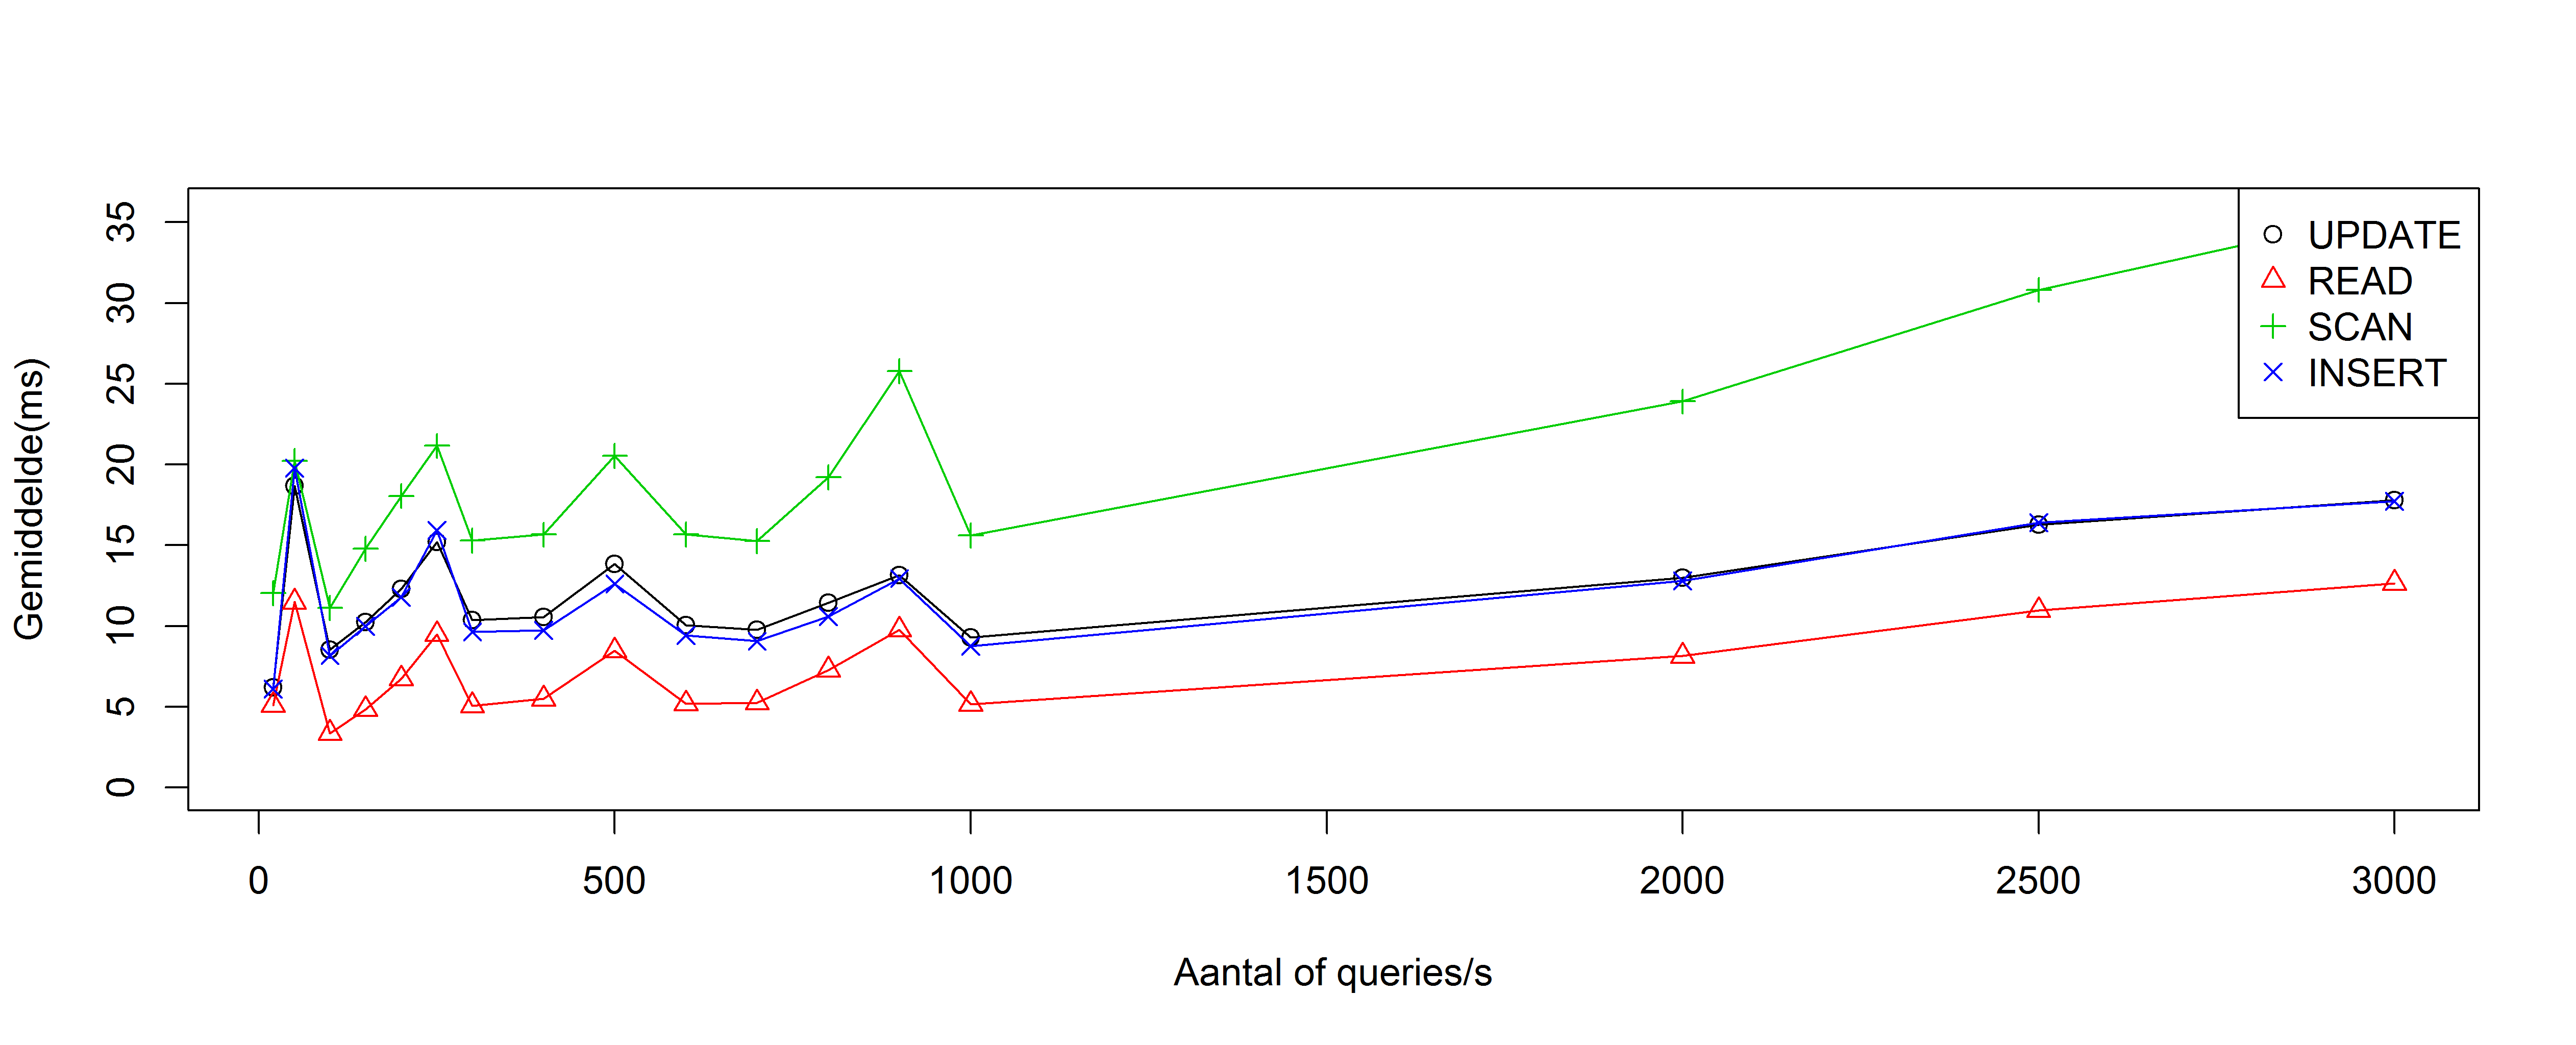
\includegraphics[width=0.8\textwidth]{img/Observaties/loadbalance-db-HBase}}
	\subfigure{\label{fig:calibratie-queriesperseconde-hbase-2} 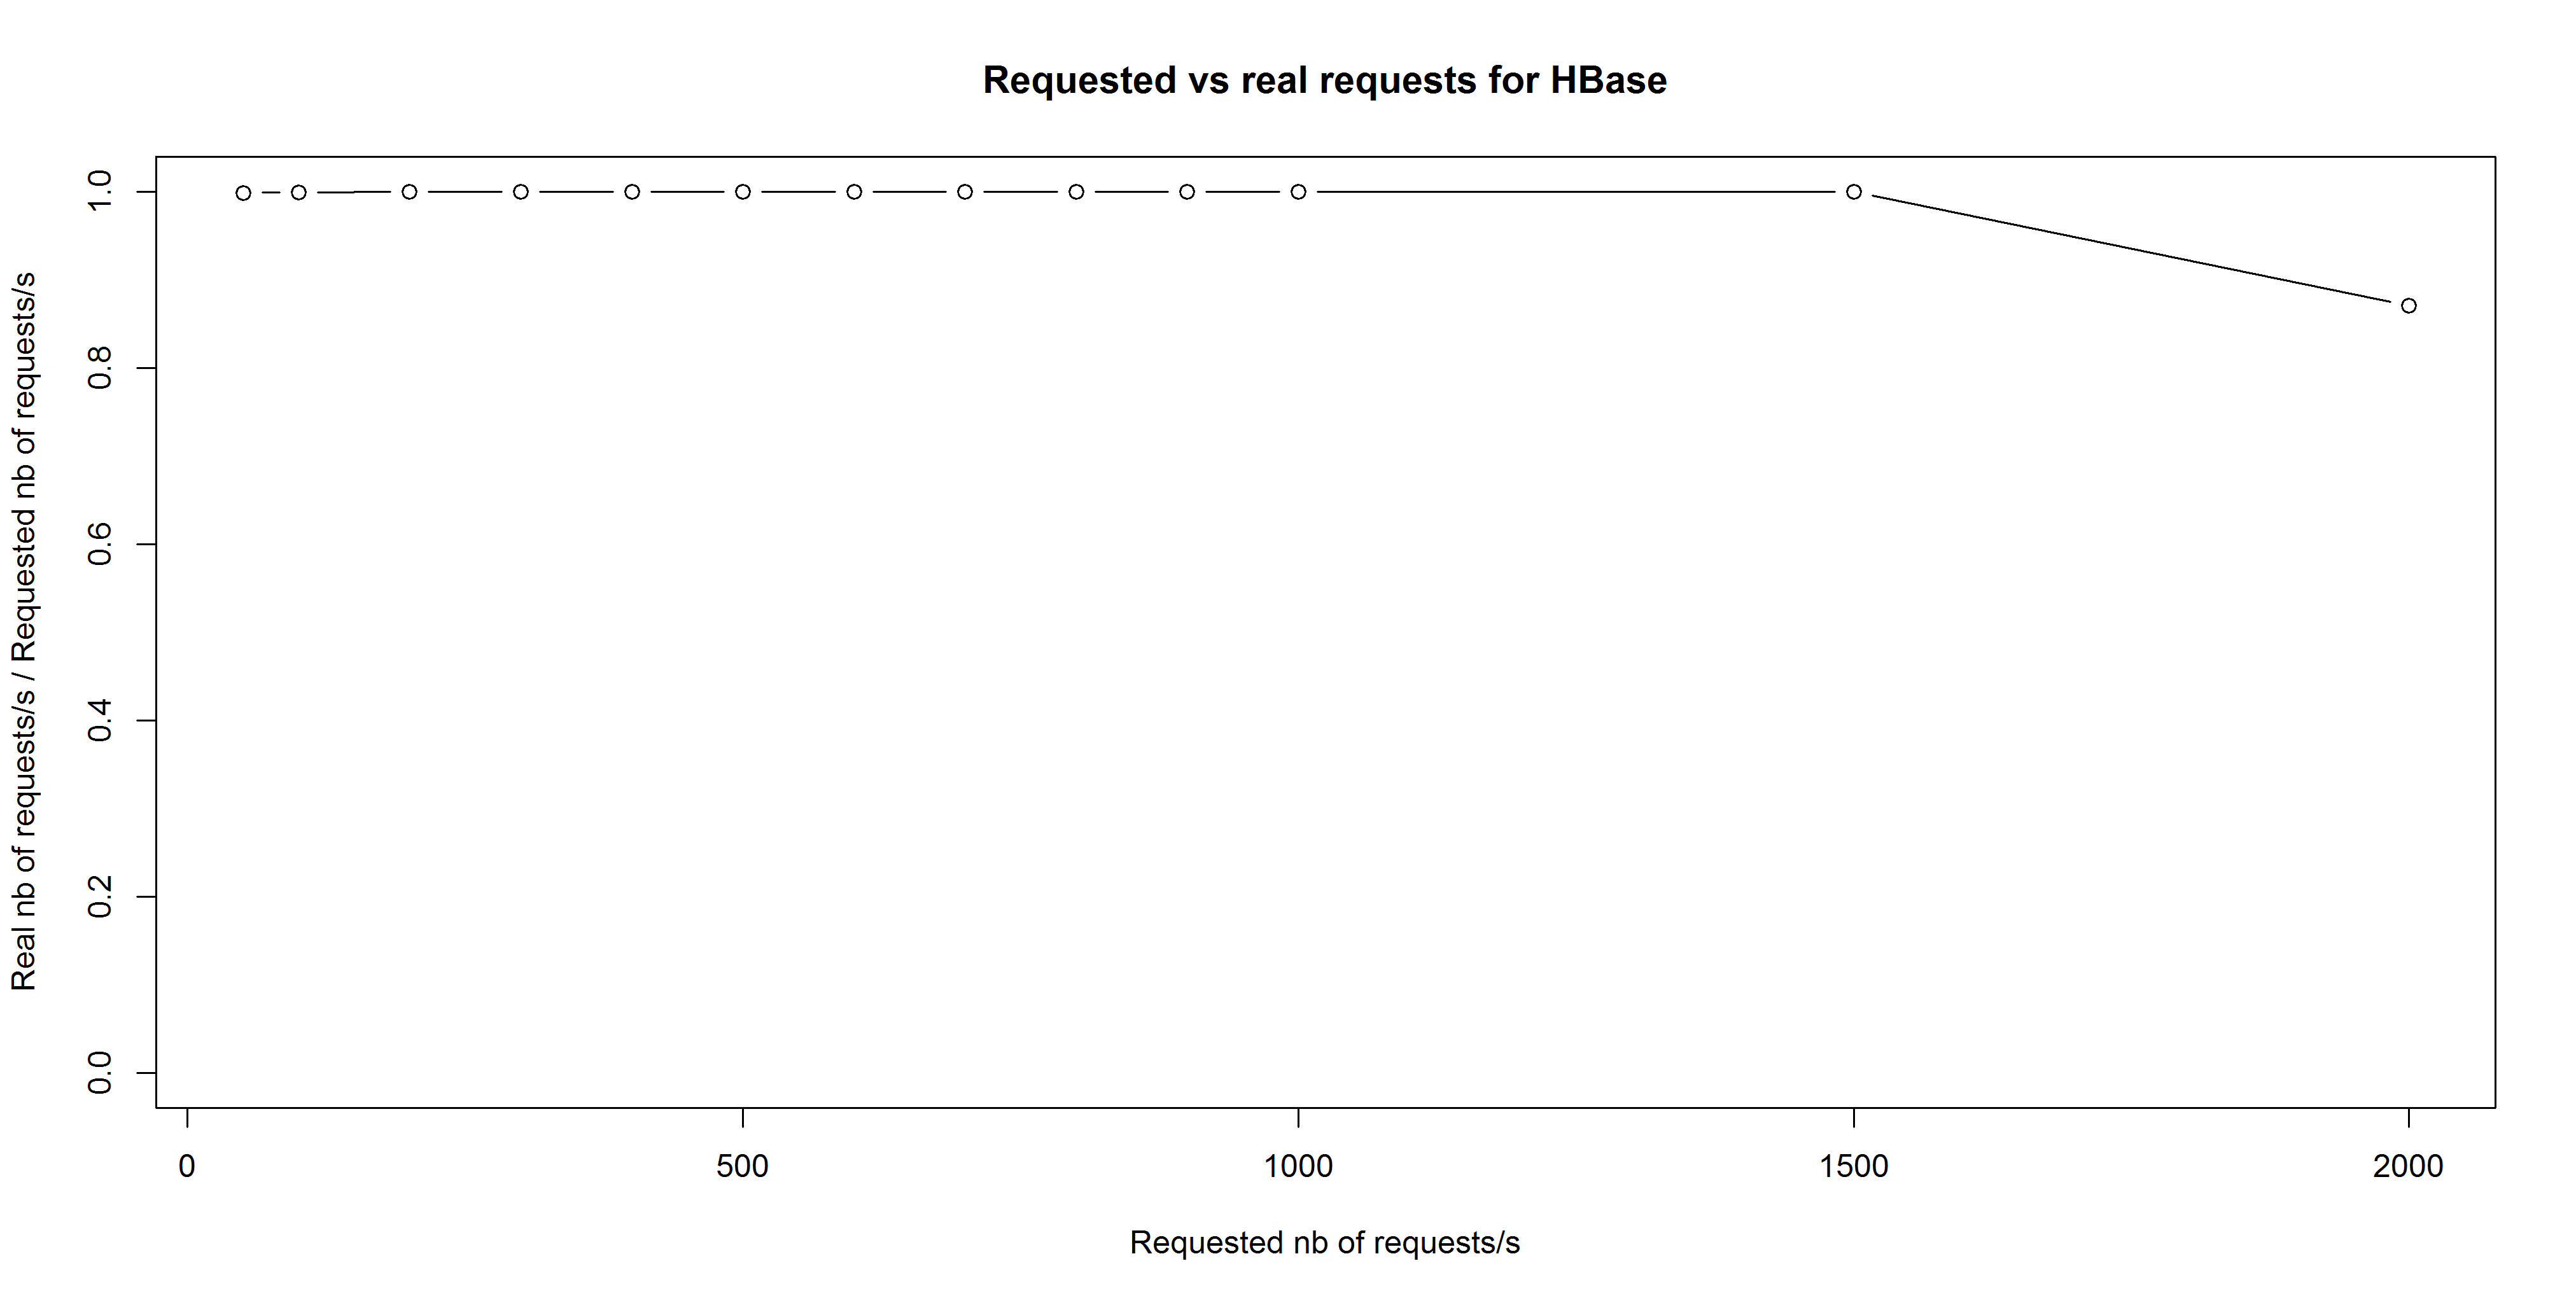
\includegraphics[width=0.8\textwidth]{img/Observaties/loadbalance-realthroughput-db-HBase}}
	\caption{Calibratie: Overzicht van de vertraging t.o.v. het theoretisch aantal aanvragen met een vergelijking hoeveel werkelijke aanvragen er waren voor HBase. }
	\label{fig:calibratie-queriesperseconde-hbase}
\end{figure}

\begin{figure}[h!] 
	\centering
	\subfigure{\label{fig:calibratie-queriesperseconde-mongodb-1} 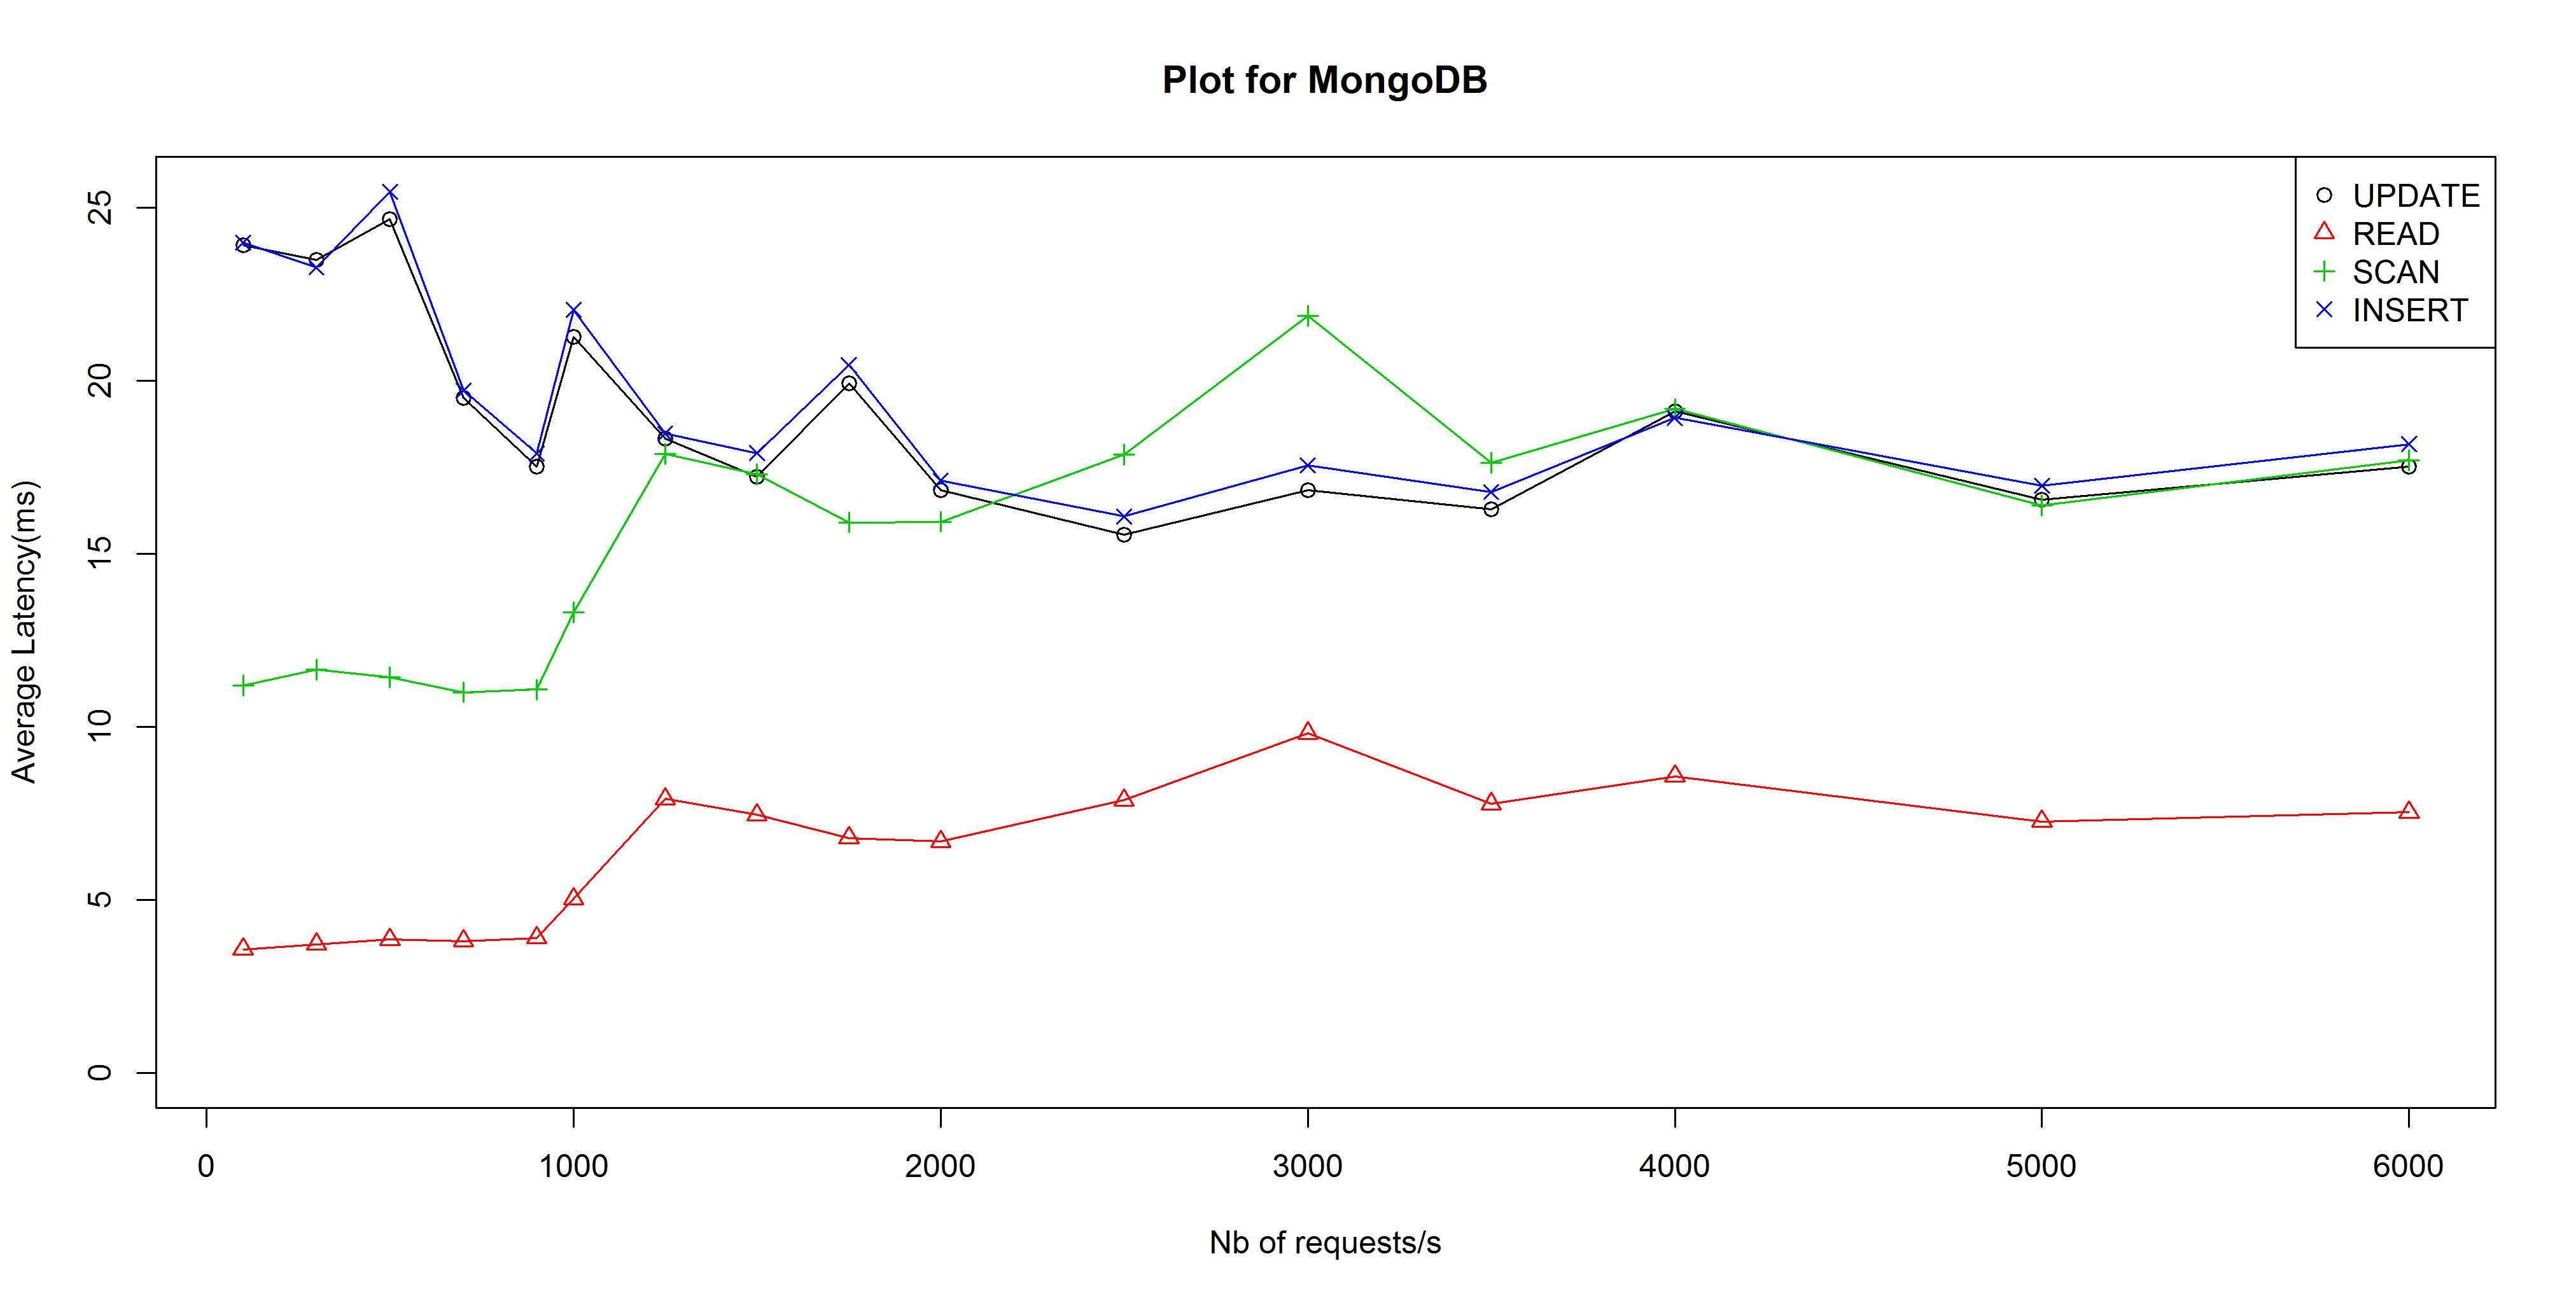
\includegraphics[width=0.8\textwidth]{img/Observaties/loadbalance-db-MongoDB}}
	\subfigure{\label{fig:calibratie-queriesperseconde-mongodb-2} 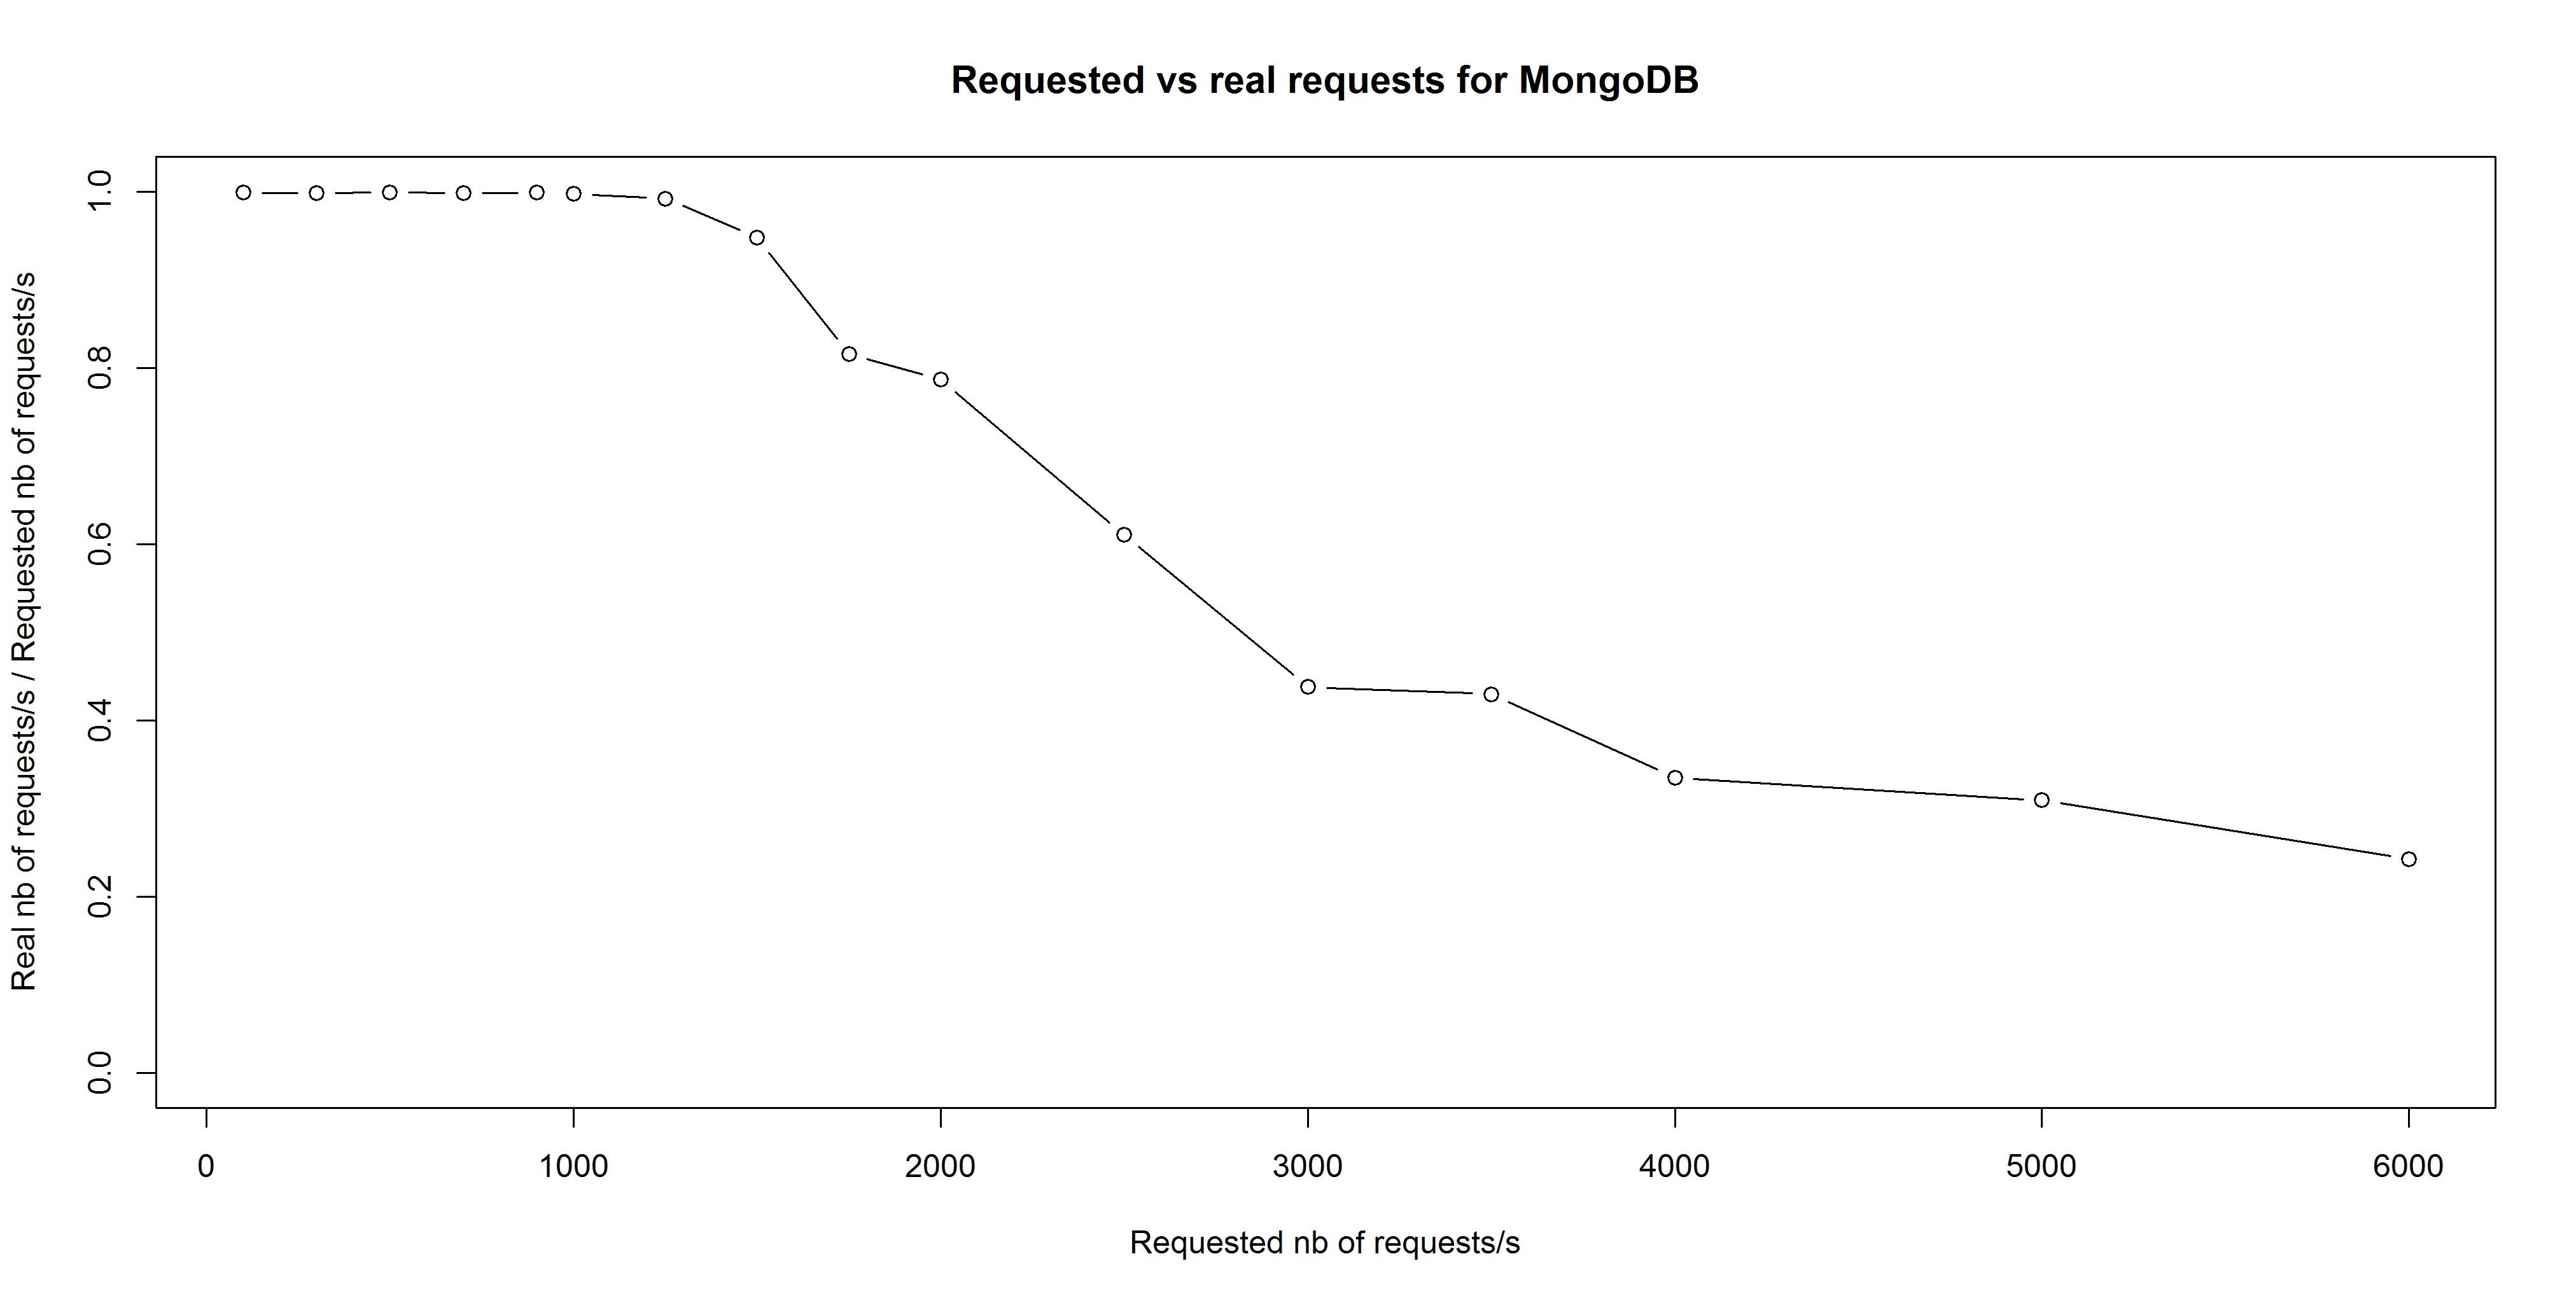
\includegraphics[width=0.8\textwidth]{img/Observaties/loadbalance-realthroughput-db-MongoDB}}
	\caption{Calibratie: Overzicht van de vertraging t.o.v. het theoretisch aantal aanvragen met een vergelijking hoeveel werkelijke aanvragen er waren voor MongoDB. }
	\label{fig:calibratie-queriesperseconde-mongodb}
\end{figure}

\begin{figure}[h!] 
	\centering
	\subfigure{\label{fig:calibratie-queriesperseconde-pgpool-ii-1} 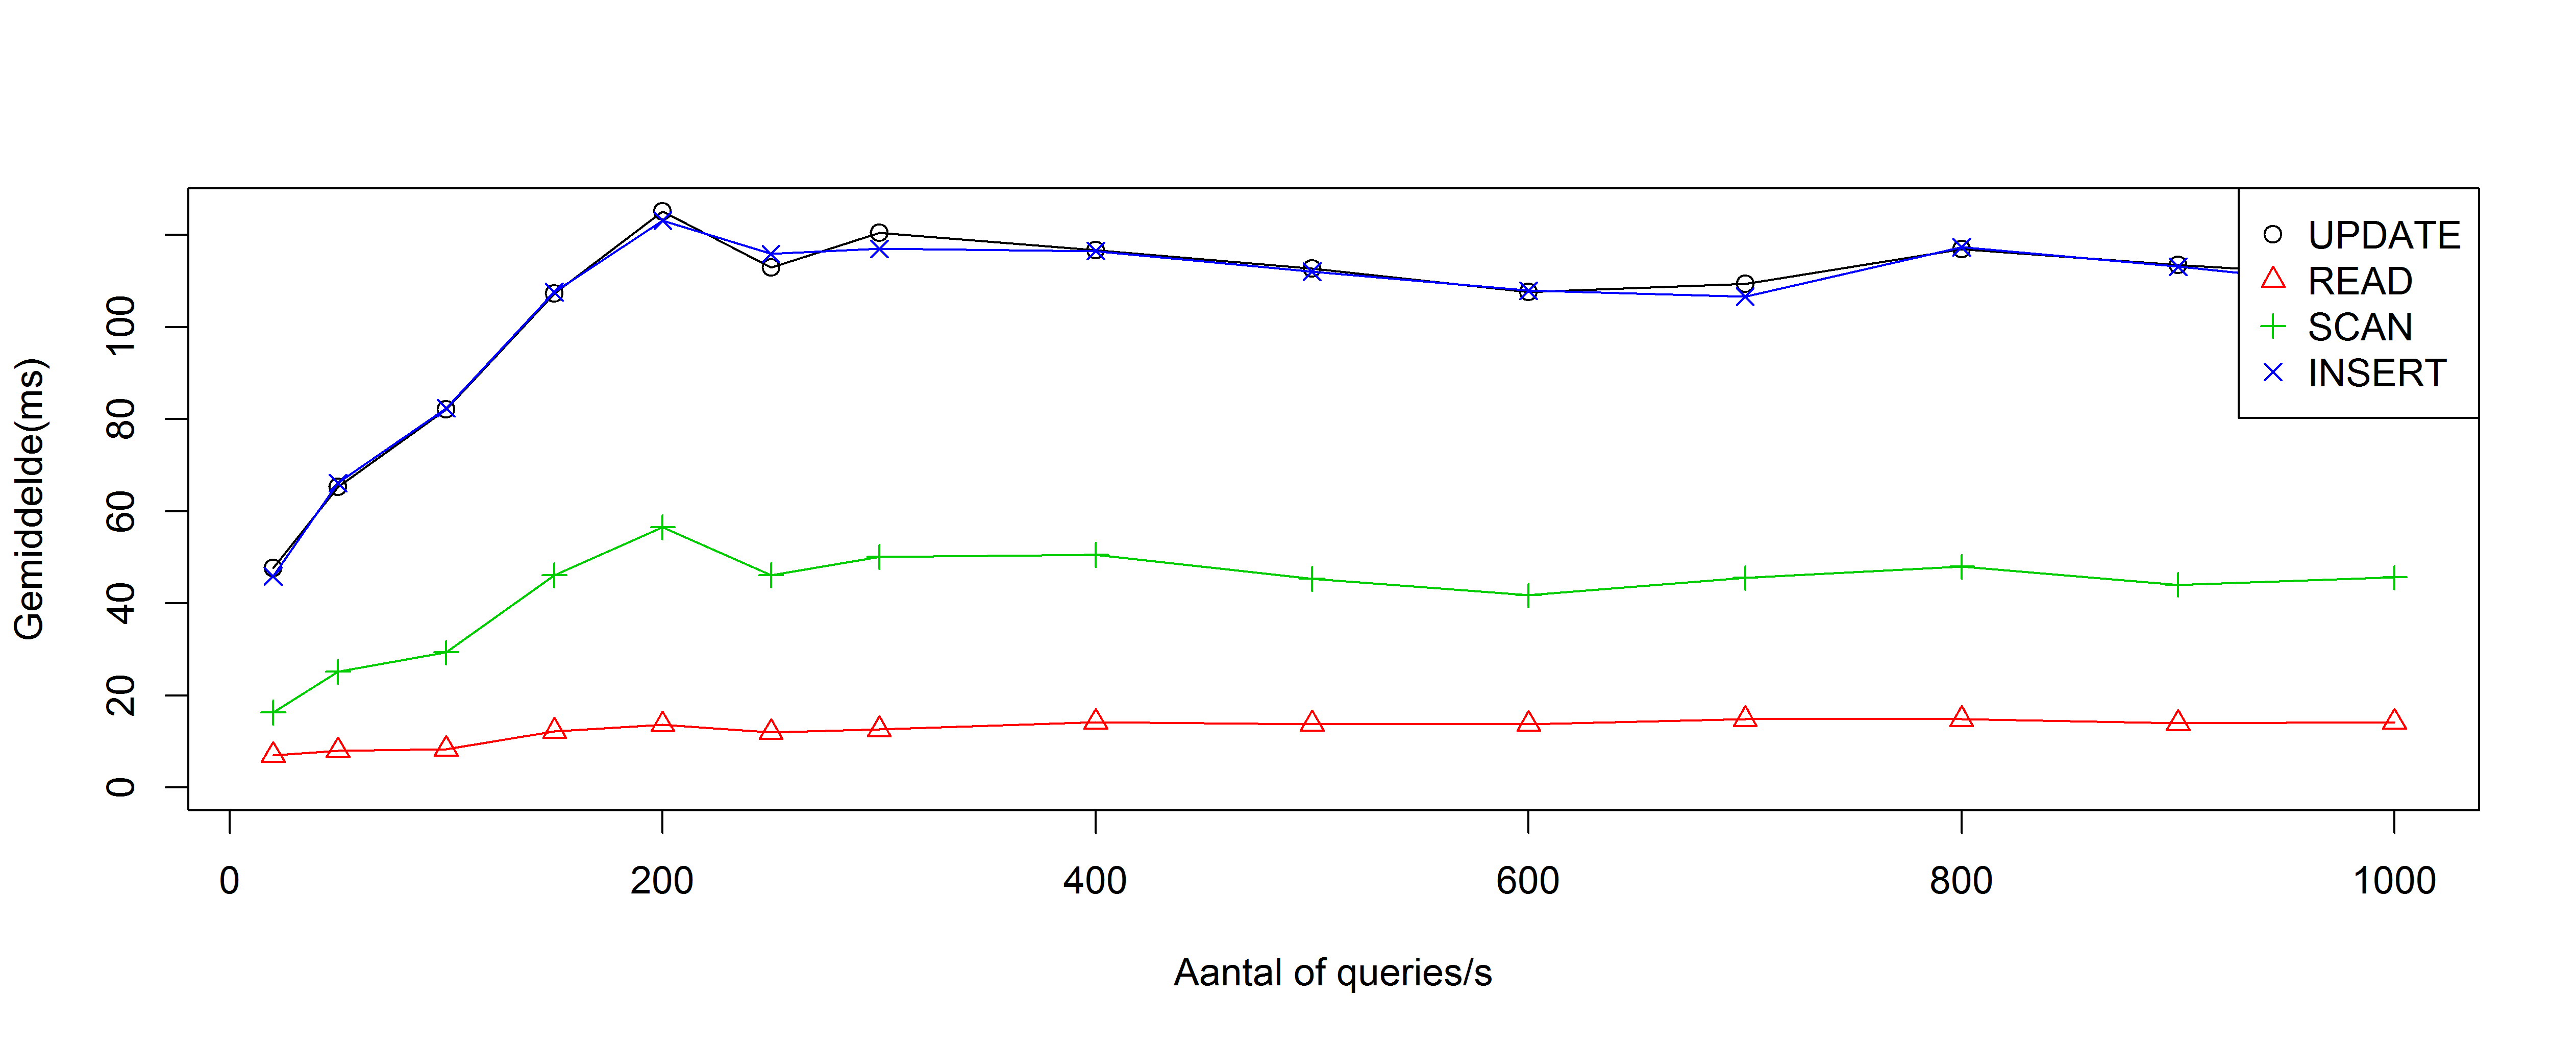
\includegraphics[width=0.8\textwidth]{img/Observaties/loadbalance-db-PostgreSQL}}
	\subfigure{\label{fig:calibratie-queriesperseconde-pgpool-ii-2} 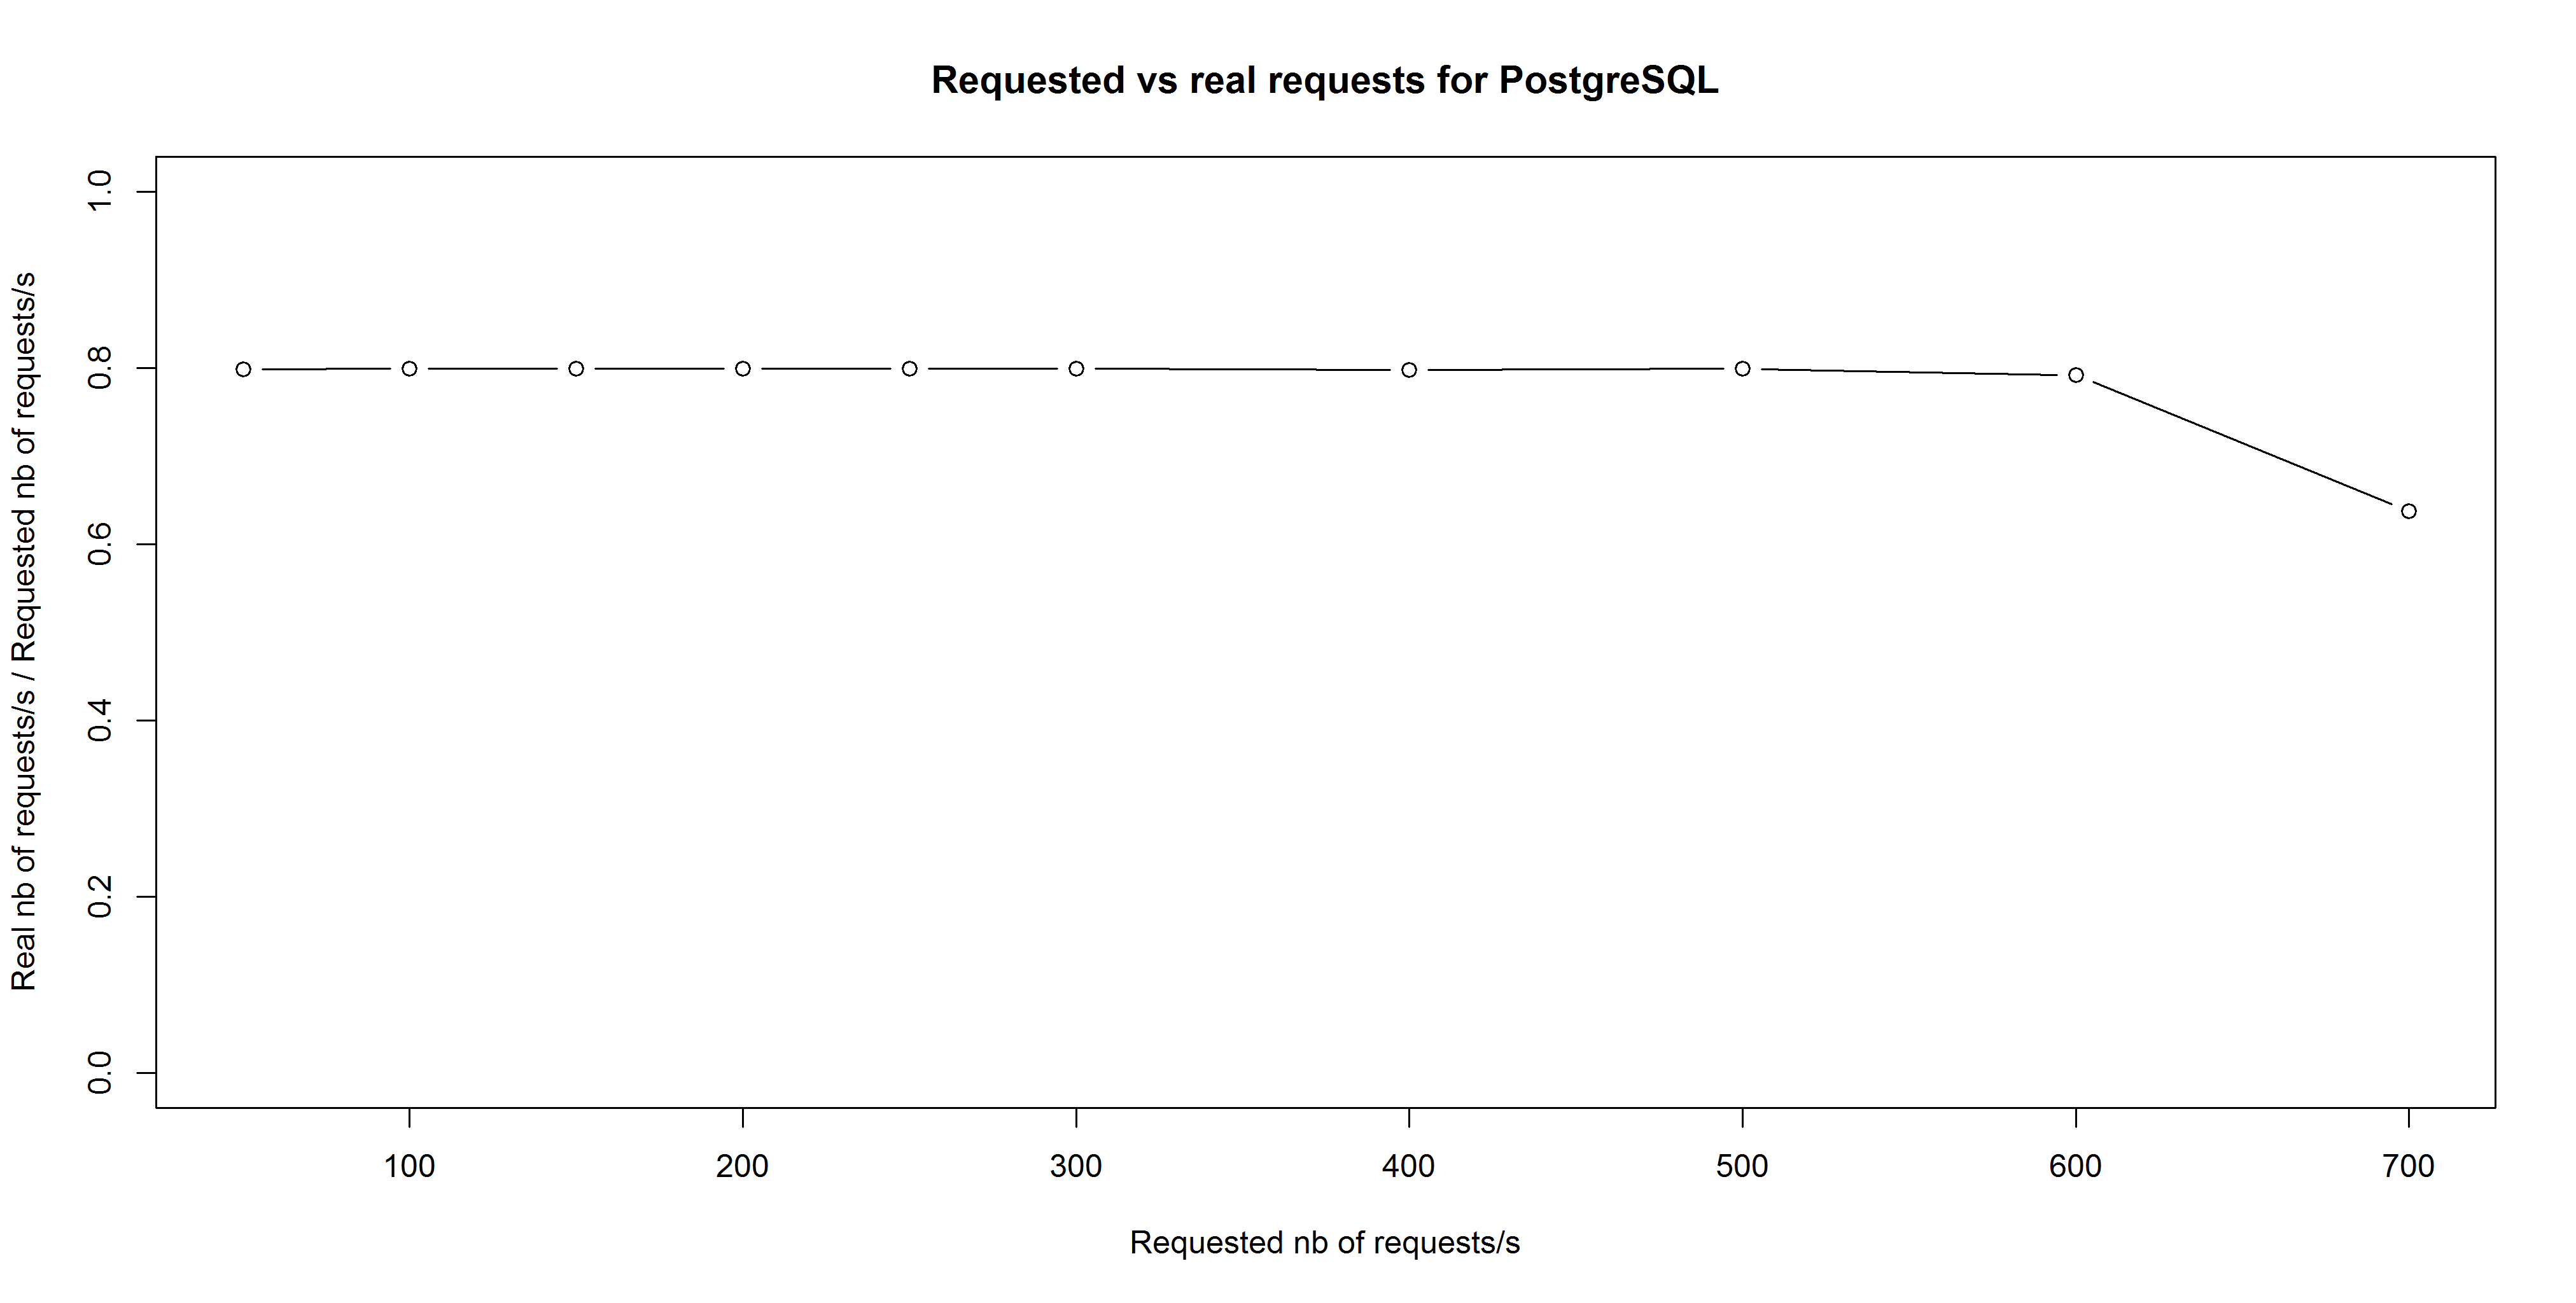
\includegraphics[width=0.8\textwidth]{img/Observaties/loadbalance-realthroughput-db-PostgreSQL}}
	\caption{Calibratie: Overzicht van de vertraging t.o.v. het theoretisch aantal aanvragen met een vergelijking hoeveel werkelijke aanvragen er waren voor Pgpool-II. }
	\label{fig:calibratie-queriesperseconde-pgpool-ii}
\end{figure}

\section{Beschikbaarheidstest}
Bij de beschikbaarheidstesten kunnen de gegevens op 3 manieren voorgesteld worden: de vertraging per query over de hele test, de vertraging tijdens het stoppen en starten van systemen of een vergelijking van de vertraging voor het stoppen, na het herstarten en tussen het stoppen en starten. 

Voor elk van de systemen is voor al de acties op de verschillende instanties data in voorhand, maar slechts enkele grafieken zullen getoond worden. Al de grafieken kunnen gevonden worden op GitHub op de link gegeven in het begin van het hoofdstuk. 

\paragraph{HBase} \todo{}

\paragraph{MongoDB} \todo{}

\paragraph{PostgreSQL} \todo{}

\section{Consistentie test}
